%% Tex spellcheck = fr_FR
\chapter{Chapter 4 : GPS Characteristics}

There is some accuracy limitations or to the \gls{gps} system. Some of them are due to the system itself, others are due to the environment and the receiver. In this chapter, we will explore some of these limitations and the solutions that have been developed to mitigate them.

\section{Environmental limitations}

The \gls{gps} accuracy can be affected by 4 main environmental factors. Even small errors in the time measurement can lead to large errors in the position calculation. We'll explore these factors and possible correction methods.

\subsection{Atmospheric effects}

The \gls{gps} signal is affected by the atmosphere. Some of these layers can change the way the signal propagates, thus affecting the time it takes for the signal to reach the receiver. The main layers that affect the signal are the ionosphere and the troposphere.

\begin{figure}[H]
	\centering
	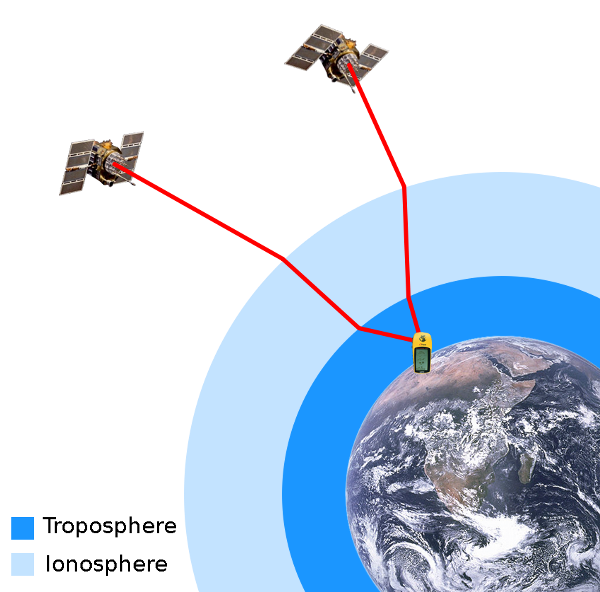
\includegraphics[width=0.5\linewidth]{atmosphere.png}
	\caption[Earth atmosphere layers deformation]{Earth atmosphere layers deformation representation Source: https://commons.wikimedia.org/ ref: URL08}
	\label{fig:earth_atmosphere}
\end{figure}

Issues with the ionosphere can be mitigated by using dual-frequency receivers. The ionosphere affects the signal by delaying the signal, this delay is proportional to the frequency of the signal. By using two different frequencies, the receiver can calculate the delay and correct the position.

There also exists some models that can predict the ionosphere delay depending on the satellites positions but these models are not perfect and can't be used in all situations.

\subsection{Multipath}

Multipath is a phenomenon that occurs when the signal is reflected by an object before reaching the receiver. This reflection can cause the signal to take a longer path to reach the receiver, thus affecting the time it takes for the signal to reach the receiver.
%fig:prn_generator
\begin{figure}[H]
	\centering
	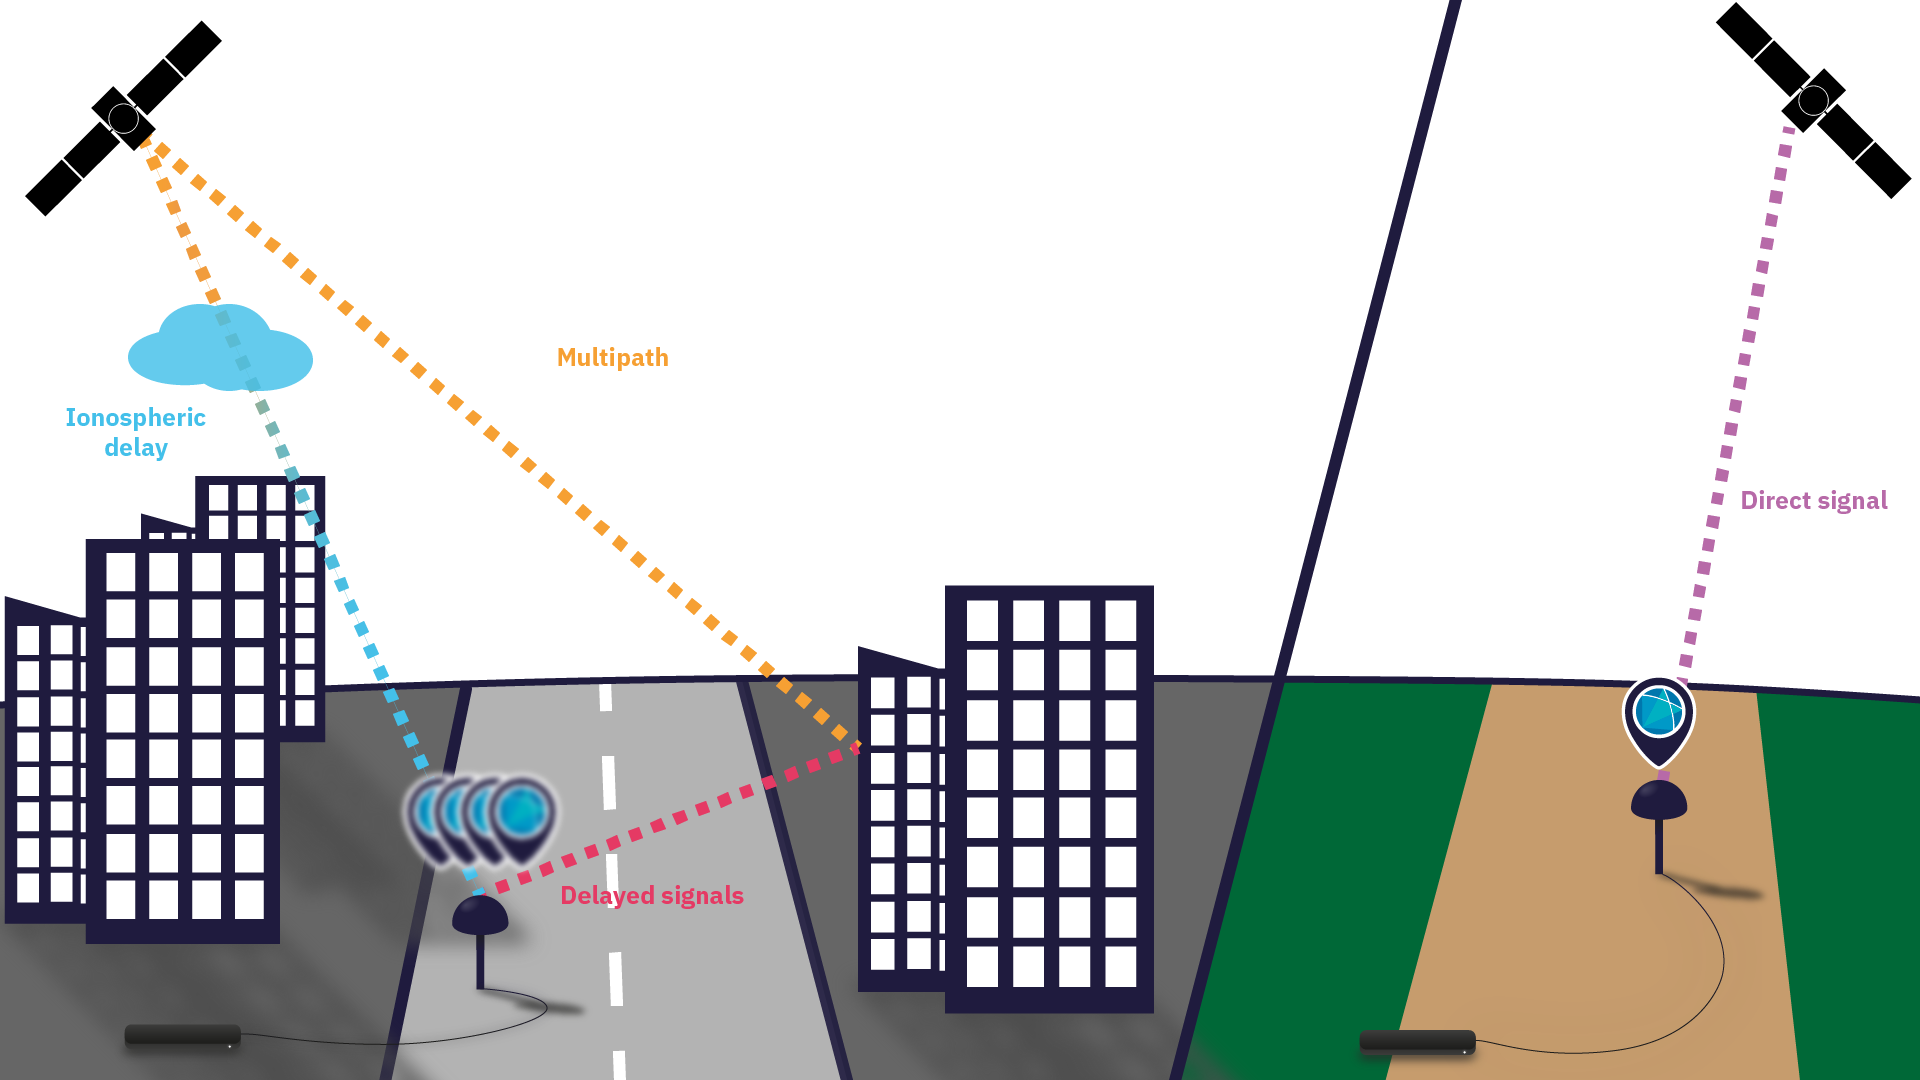
\includegraphics[width=0.5\linewidth]{multipath.png}
	\caption[Multipath explicative diagram]{Multipath explicative diagram Source: https://syntony-gnss.com/ ref: URL08}
	\label{fig:multipath}
\end{figure}

In the example in Figure \ref{fig:multipath}, we can see a direct signal on the right that directly goes to a receiver, and a reflected signal on the left that goes to the receiver after being reflected by a building. This reflected signal will take longer to reach the receiver, thus affecting the time measurement, and thus the position calculation.

This issue is still a problem today, and there are no perfect solutions to mitigate it because we're not able to predict the position of all the reflecting objects.


\subsection{Ephemeris error}

The \gls{gps} system uses the position of the satellites to calculate the position of the receiver. This means that the actual position of the satellite is important. However the position and orbital parameters and corrections made by the satellites are not absoulutely perfect and can have some errors.

There is a system in place to correct these errors, the \gls{sbas} system. This system uses ground stations to monitor the position of the satellites and to send corrections to the satellites. These corrections are then broadcasted to the receivers.


\subsection{Satellite clock drift}

Even though the \gls{sv}s are equipped with atomic clocks, they are not perfect and can drift a little but this drift is actually compensated by software. We will also mention that the relativistic effects also have to be taken into account when calculating the time difference between the receiver and the satellite (The time in the satellite reference frame is different than the time in the receiver reference frame since it's moving at a different speed and is in a different gravitational field).


\section{Augmentation systems}

The base \gls{gps} with only the L1 \gls{ca} code has an accuracy of about \textbf{10 meters.} This is not enough for some applications, so some augmentation systems have been developed to improve the accuracy of the system. One limitation is that the receiver often needs to be compatible with these systems to use them.

\subsection{Differential GPS}

The \gls{dgps} is a system that uses a reference ground station\footcite{noauthor_23_nodate} located at a known position to calculate the errors in the \gls{gps} system. The ground station knows exactly where it is, so it can determine the errors of the received signals and then broadcast these errors to the receivers. The receivers can then correct their position using these errors. This augmentation needs ground stations to be installed at maximum 400 km from the receiver we want to augment.

\textbf{The final accuracy with \gls{dgps} is about 3cm.}


\subsection{RTK}

The \gls{rtk} works on the same principle as the \gls{dgps}. It's usually a complete system with 2 devices, a base station and a rover. The base station gets its position from a known source and then calculates the errors in the \gls{gps} system. The base station then sends these errors to the rover, which can then correct its position using these errors. The correction is usually given via \gls{rf} or \gls{gsm}.



\begin{figure}[H]
	\centering
	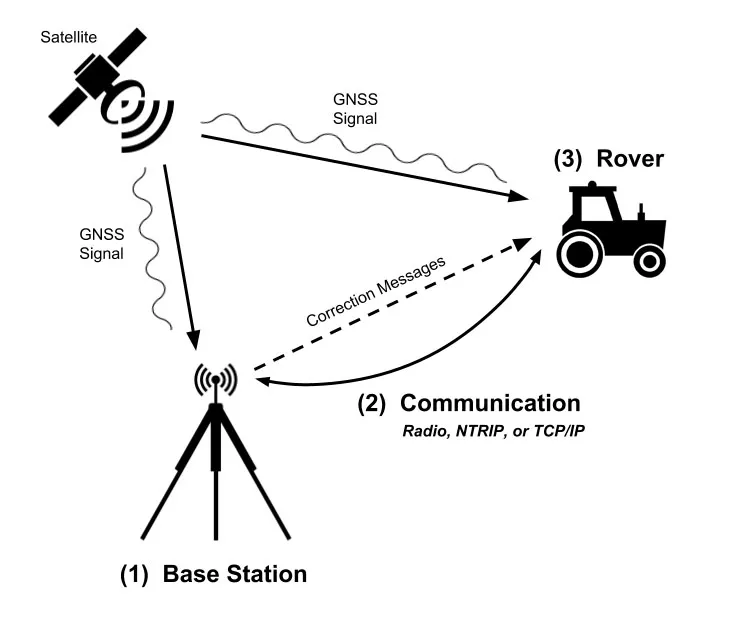
\includegraphics[width=0.5\linewidth]{rtk_diagram.png}
	\caption[RTK Diagram]{RTK Diagram Source: https://i0.wp.com ref: URL10}
	\label{fig:rtk}
\end{figure}

In \ref{fig:rtk} figure, we can observe a fixed base station, receiving GNSS signal and sending corrections to the rover. The rover receive both GNSS signals and the corrections from the base station.

\begin{figure}[H]
	\centering
	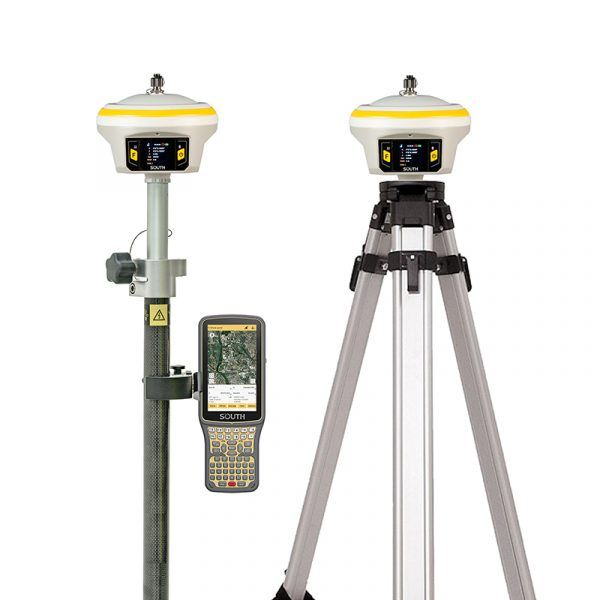
\includegraphics[width=0.5\linewidth]{rtk_example.jpg}
	\caption[Real RTK system]{Photo of an existing RTK system (South INNO7 rover base set) Source: https://globalgpssystems.com ref: URL11}
	\label{fig:rtk_example}
\end{figure}

%\textbf{The final accuracy with \gls{rtk} is about 1cm.\footcite{noauthor_how_2020}}

\subsection{SBAS}

The \gls{sbas} uses a network of ground stations to monitor the \gls{gps} system and to send corrections to Geostationary satellites \footnote{A geostationary satellite is a satellite that is placed in a geostationary orbit, this means that the satellite is always at the same position relative to the Earth.} that then broadcast these corrections to the receivers. This system is used to improve the accuracy of the \gls{gps} system in a large area, like a continent.

There actually is four main \gls{sbas}:

\begin{itemize}
	\item \gls{waas} for North America
	\item \gls{egnos} for Europe
	\item \gls{msas} for Japan
	\item \gls{gagan} for India
\end{itemize}

\begin{figure}[H]
	\centering
	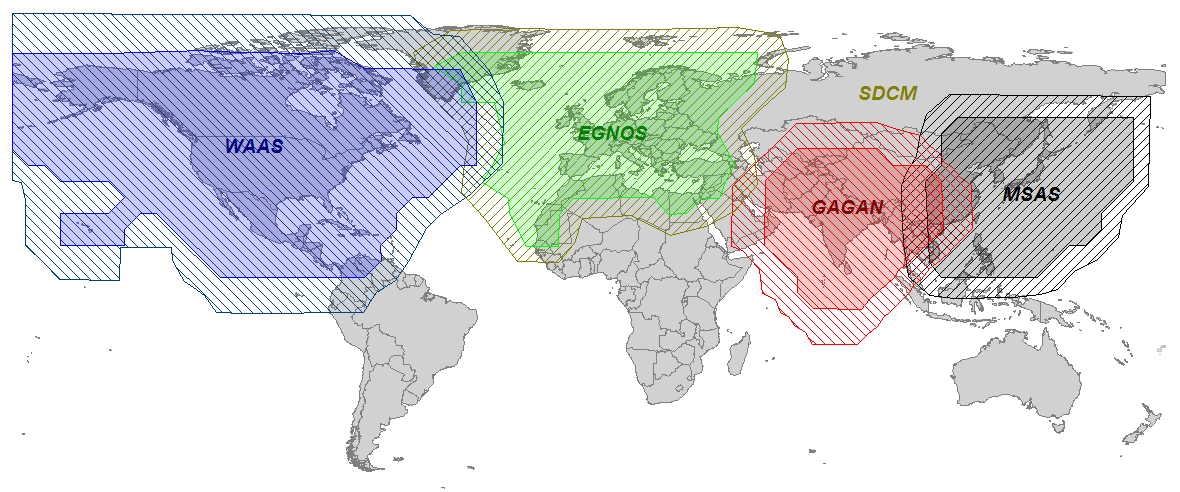
\includegraphics[width=1\linewidth]{SBAS.png}
	\caption[Main SBAS Systems]{Map of the main \gls{sbas} systems  Source: https://www.reseau-teria.com ref: URL12}
	\label{fig:sbas}
\end{figure}